% !TeX root = main.tex
\subsection{Assignment 3: Time scaling}

A detailed report is present at \href{https://github.com/TheProjectsGuy/IS_RPN22-EC9.404/tree/main/assignment-2b-over-9000}{TheProjectsGuy/IS\_RPN22-EC9.404}

\subsubsection{Constant Time Scaling}

Constant time scaling is implemented using the equation below

\begin{equation}
    \dot{x} (\tau) = k \: \dot{x}(t)
\end{equation}

The results for this are shown in figure \ref{fig:rb-cts-exp1}.

\begin{figure}[ht]
    \centering
    \begin{subfigure}[b]{0.4\textwidth}
        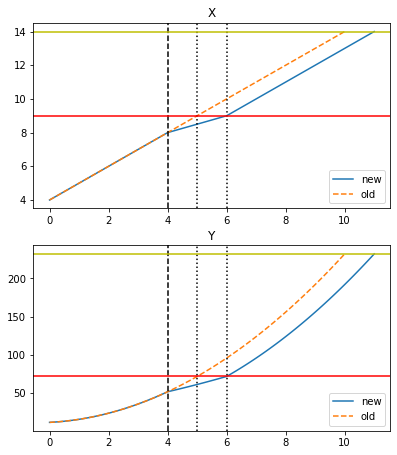
\includegraphics[width=\textwidth]{rb-cts-holo.png}
        \caption{Time scaling}
    \end{subfigure}
    \begin{subfigure}[b]{0.3\textwidth}
        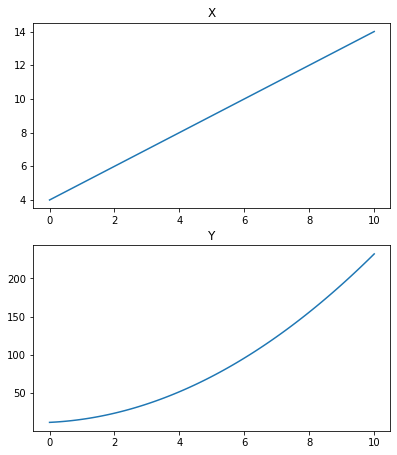
\includegraphics[width=\textwidth]{rb-cts-holo-origxy.png}
        \caption{Original}
    \end{subfigure}
    \begin{subfigure}[b]{0.25\textwidth}
        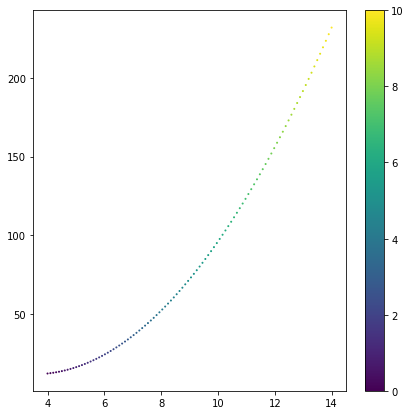
\includegraphics[width=\textwidth]{rb-cts-holo-xy.png}
        \caption{XY}
    \end{subfigure}
    \caption{Time scaling}
    \label{fig:cts-rb-holo}
    \small
        The variables $X$ and $Y$ are functions of time. The time scaling is applied from $4$ to $5$ seconds, with $k=0.5$ (the new end of time scaling will therefore happen at $6$ seconds).

        In left figure, it is apparent that the velocities have decreased to half in the time scaling period, while the duration has doubled.

        The center and right figures show the original trajectory ($X$ and $Y$ as function of time in center, and $X$ vs. $Y$ plot in the right).
\end{figure}

\begin{figure}[ht]
    \centering
    \begin{subfigure}[b]{0.3\textwidth}
        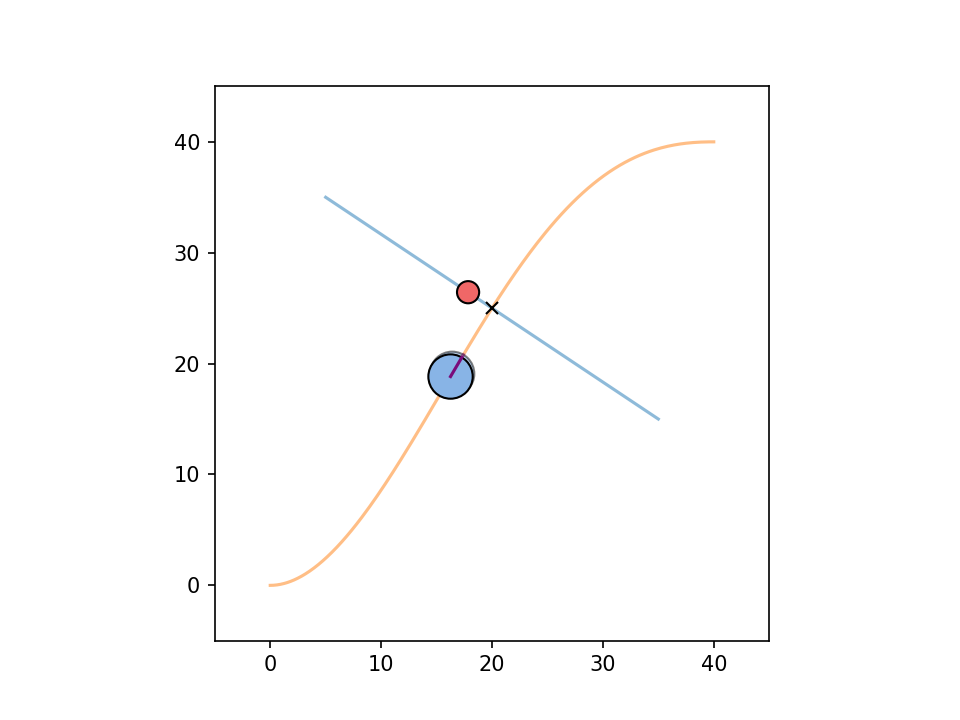
\includegraphics[width=\textwidth]{res1-ts-start.png}
        \caption{Start}
    \end{subfigure}
    \begin{subfigure}[b]{0.3\textwidth}
        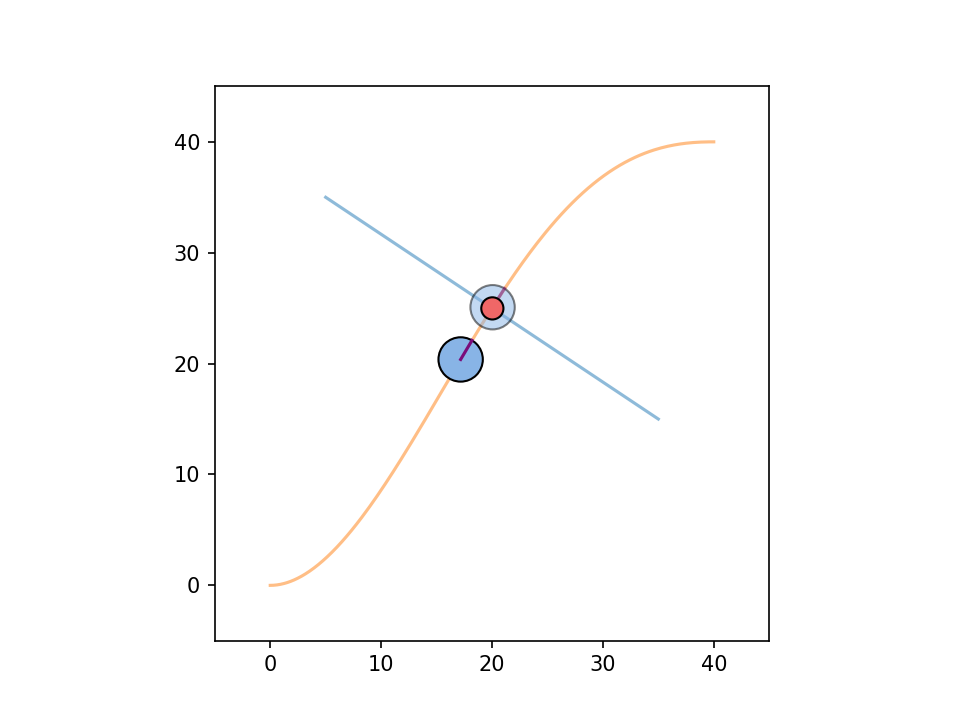
\includegraphics[width=\textwidth]{res1-ts-colav.png}
        \caption{Collision avoidance}
    \end{subfigure}
    \begin{subfigure}[b]{0.3\textwidth}
        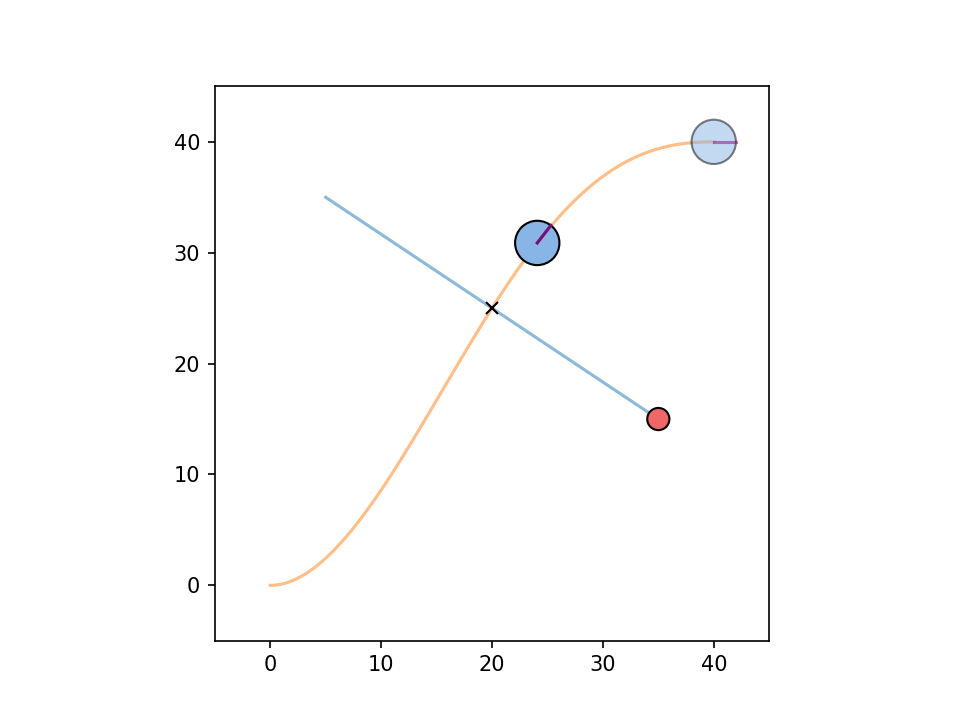
\includegraphics[width=\textwidth]{res1-ts-end.png}
        \caption{End}
    \end{subfigure}
    \caption{Rule-based constant time-scaling}
    \label{fig:rb-cts-exp1}
\end{figure}

\subsubsection{Collision cone based constant time-scaling}

A collision cone is comprised of the relative velocities of the robot (with reference to an obstacle) that will lead to a collision in the future. This is demonstrated in the figure \ref{fig:cc-cts-imgs}.

\begin{figure}[ht]
    \begin{subfigure}[b]{0.24\textwidth}
        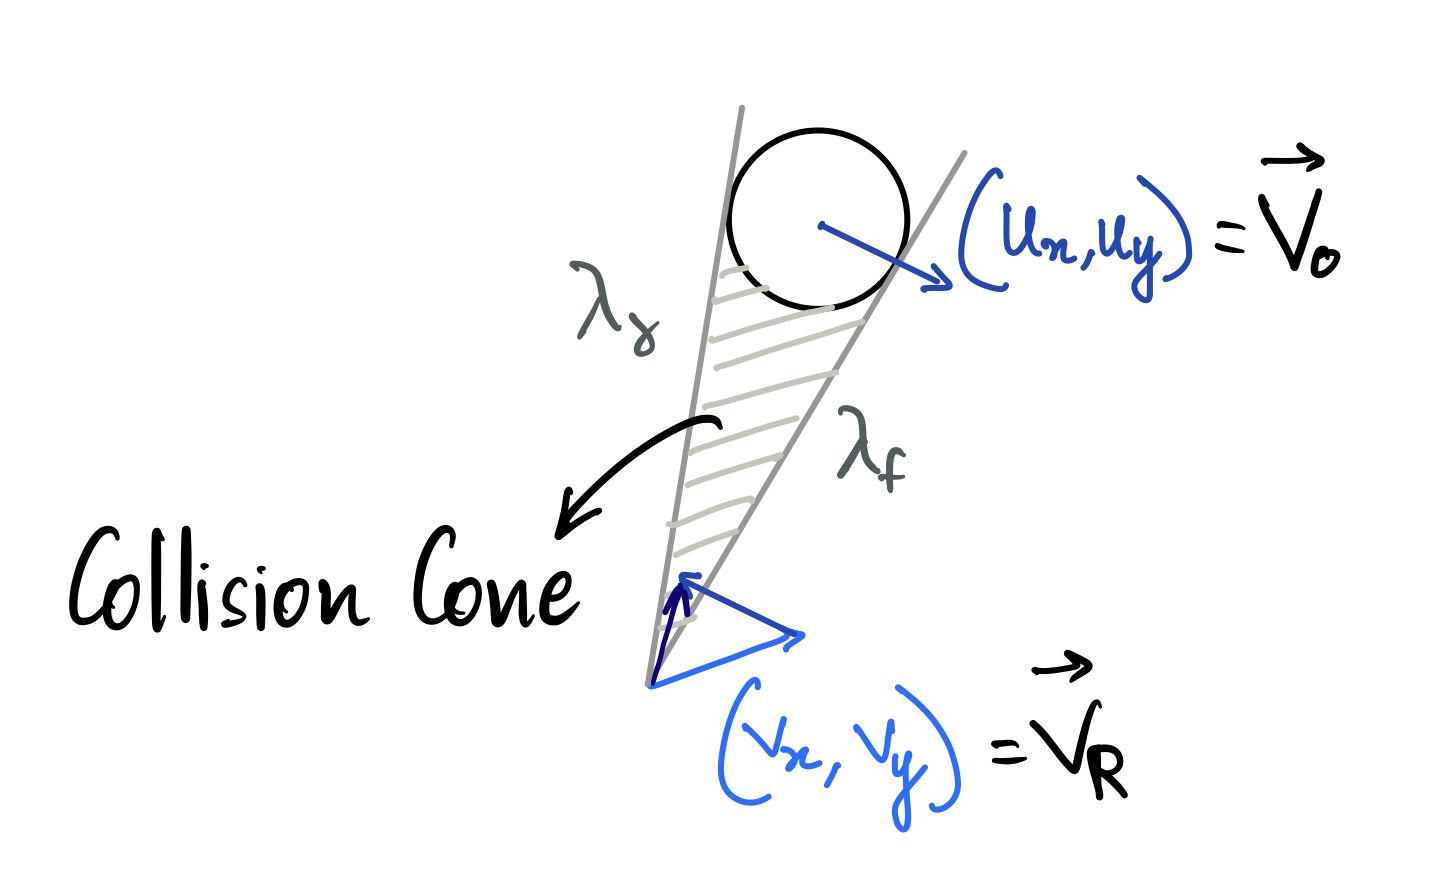
\includegraphics[width=\textwidth]{cc-img1.PNG}
        \caption{Collision Cone}
        \label{fig:sfig-cc-cts}
    \end{subfigure}
    \begin{subfigure}[b]{0.24\textwidth}
        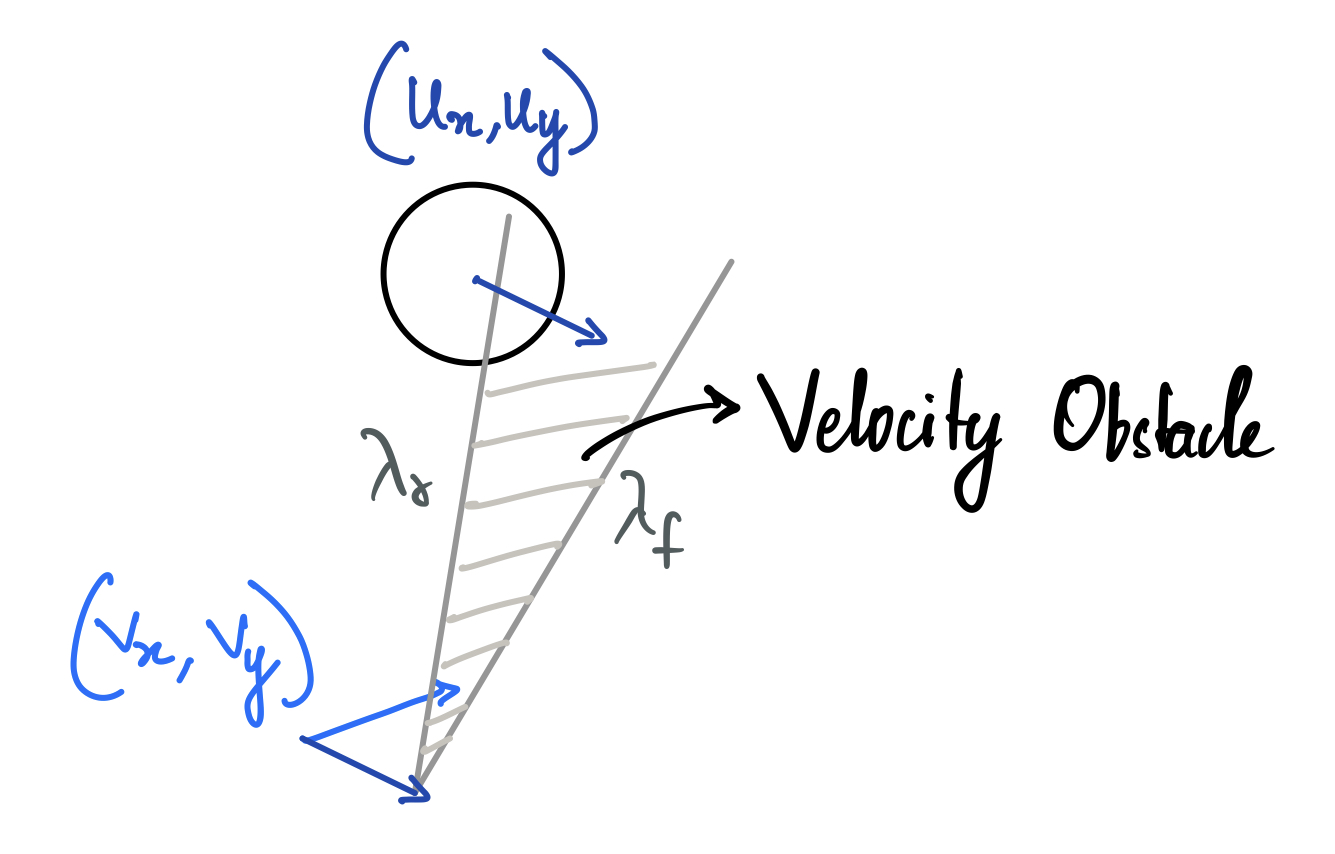
\includegraphics[width=\textwidth]{cc-img2.PNG}
        \caption{Velocity Obstacle}
        \label{fig:sfig-vo-cts}
    \end{subfigure}
    \begin{subfigure}[b]{0.24\textwidth}
        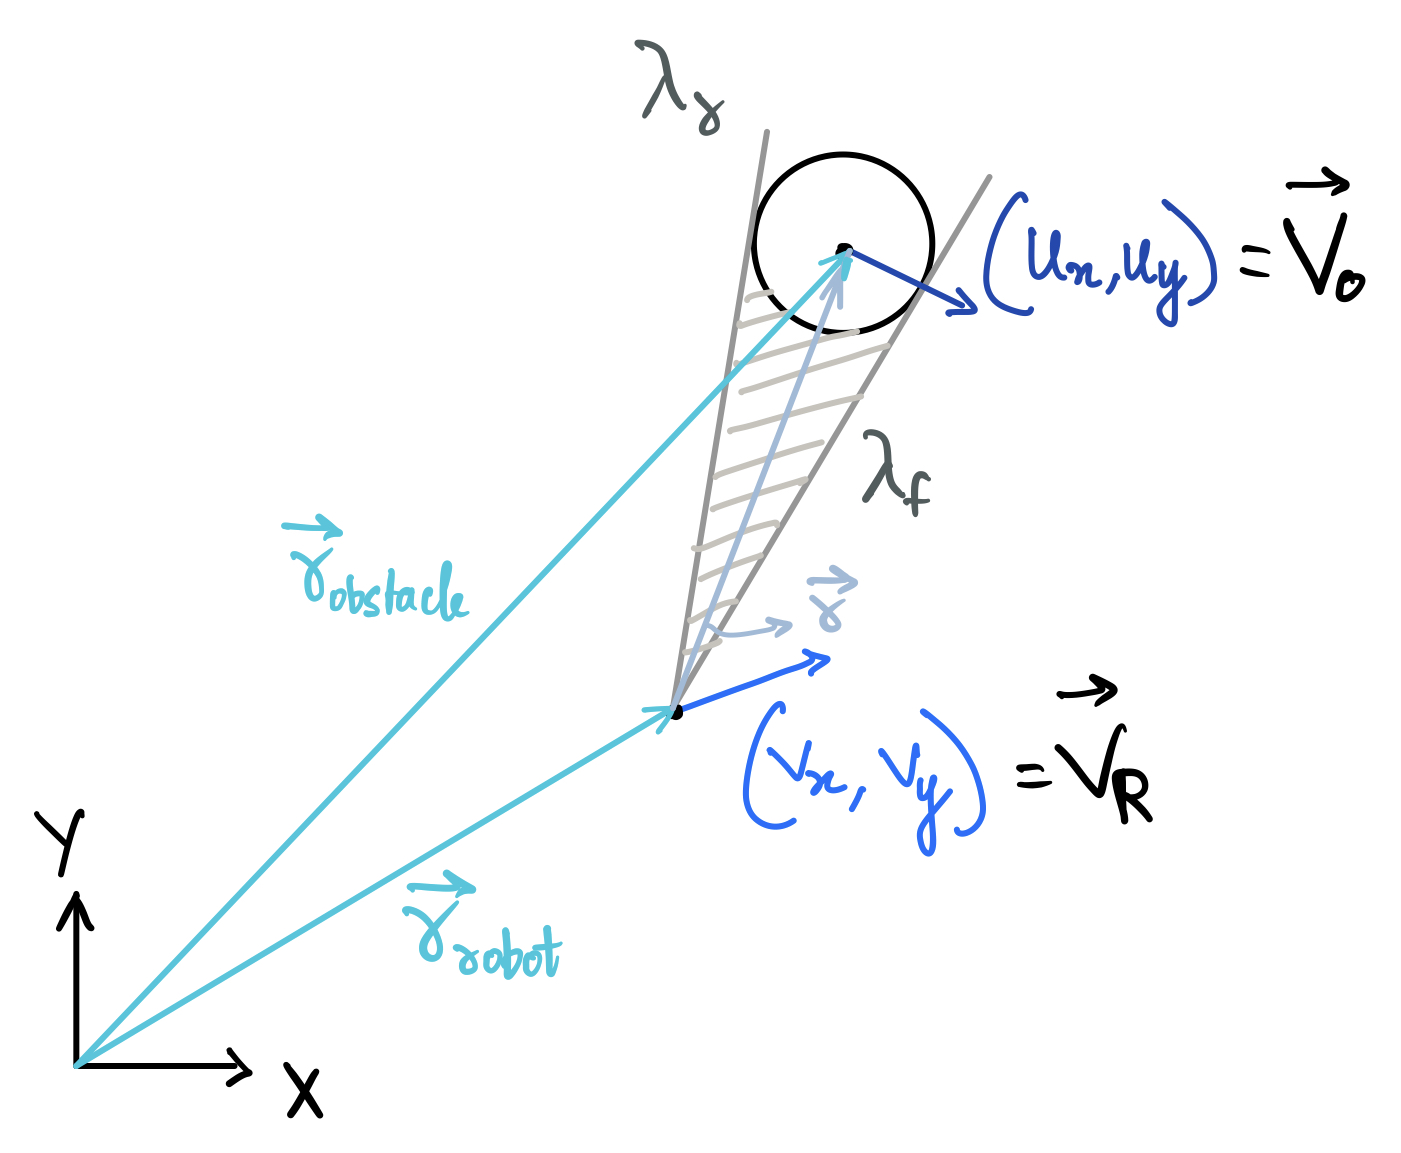
\includegraphics[width=\textwidth]{cc-img3.PNG}
        \caption{Environment}
        \label{fig:sfig-env-cts}
    \end{subfigure}
    \begin{subfigure}[b]{0.24\textwidth}
        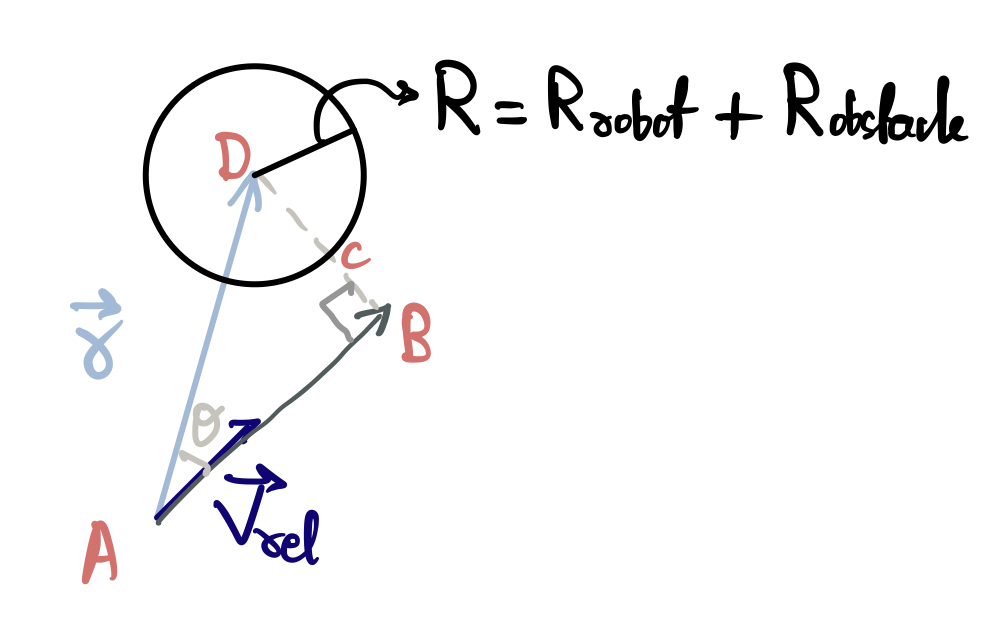
\includegraphics[width=\textwidth]{cc-img4.PNG}
        \caption{Avoiding collision}
        \label{fig:sfig-ac-cts}
    \end{subfigure}
    \caption{Collision Cone}
    \label{fig:cc-cts-imgs}
    \small
        The velocity of obstacle is $\overrightarrow{V}_{O} = (u_x, u_y)$. The velocity of obstacle is $\overrightarrow{V}_{R} = (v_x, v_y)$. THe radius of robot is $R_{robot}$ and the radius of obstacle is $R_{obstacle}$. The obstacle is diluted to $R = R_{robot} + R_{obstacle}$ while the robot is reduced to a point.
        After time scaling, the velocity of the robot becomes scaled by a factor of $s$, that is, the time scaled robot velocity is $\vec{V}_{R} = (s\dot{x}_1, s\dot{y}_1)$.
\end{figure}

We can formulate the following to avoid a collision

\begin{align*}
    \textup{DB} \ge \textup{DC} \Rightarrow
    \textup{DB}^2 \ge R^2 \Rightarrow
    \textup{AD}^2 - \textup{AB}^2 \ge R^2
    &&
    \vec{r}_{obstacle} = \vec{r}_{robot} + \vec{r} \Rightarrow 
    \vec{r} = \vec{r}_{obstacle} - \vec{r}_{robot}
    \\
    \textup{AB} = \left \| \vec{r} \right \| \cos(\theta) = \frac{\vec{V}_{rel} \cdot \vec{r}}{\left \| \vec{V}_{rel} \right \|}
    \Rightarrow \textup{AB}^2 = \left [ \frac{\vec{V}_{rel} \cdot \vec{r}}{\left \| \vec{V}_{rel} \right \|} \right ]^2
    &&
    \textup{AD} = \left \| \vec{r} \right \| \Rightarrow \textup{AD}^2 = \left \| \vec{r} \right \|^2
\end{align*}

\begin{align*}
    \vec{V}_{rel} = \vec{V}_{R} - \vec{V}_{O} = (s\dot{x}_1 - \dot{x}_2, s\dot{y}_1 - \dot{y}_2)
    &&
    \vec{r} = \vec{r}_{obstacle} - \vec{r}_{robot} = (x_2 - x_1, y_2 - y_1) \\
    \textup{AD}^2 - \textup{AB}^2 \ge R^2 \Rightarrow 
    \left \| \vec{r} \right \|^2 - \left [ \frac{\vec{V}_{rel} \cdot \vec{r}}{\left \| \vec{V}_{rel} \right \|} \right ]^2 \ge R^2
    &&
    \left \| \vec{r} \right \|^2 - \left [ \frac{\vec{V}_{rel} \cdot \vec{r}}{\left \| \vec{V}_{rel} \right \|} \right ]^2 - R^2 \ge 0
    \\
    \vec{V}_{rel} \cdot \vec{r} = (s\dot{x}_1 - \dot{x}_2) (x_2 - x_1) + (s\dot{y}_1 - \dot{y}_2) (y_2 - y_1)
    &&
    \left \| \vec{V}_{rel} \right \| = \sqrt{\left( s\dot{x}_1 - \dot{x}_2 \right)^2 + \left( s\dot{y}_1 - \dot{y}_2 \right)^2}
\end{align*}

We get the following final inequality for the scaling factor $s$.

\begin{align}
    (x_1 - x_2)^2 + (y_1 - y_2)^2 - R^2 - \frac{\left( (s\dot{x}_1 - \dot{x}_2) (x_2 - x_1) + (s\dot{y}_1 - \dot{y}_2) (y_2 - y_1) \right)^2}{\left( s\dot{x}_1 - \dot{x}_2 \right)^2 + \left( s\dot{y}_1 - \dot{y}_2 \right)^2} \ge 0
    \label{eq:cc-cts-rawineq}
\end{align}

We represent this equation in the form $a s^2 + b s + c \ge 0$. This gives us the following solution space (set) for $s$

\begin{equation}
    S_{sol} = \left\{\begin{matrix}
        [s_{min}, \infty) \cap \left ( (-\infty, \gamma_1] \cup [\gamma_2, \infty) \right ) && a > 0,\, d > 0 \\
        [s_{min}, \infty) && a > 0,\, d < 0 \\
        [s_{min}, \infty) \cap [\gamma_1, \gamma_2] && a < 0 ,\, d > 0 \\
        \phi && a < 0 ,\, d < 0
    \end{matrix}\right.
    \label{eq:cc-cts-solspace-s}
\end{equation}

Where

\begin{align*}
    d = b^2 - 4ac
    &&
    \gamma_1 = \frac{-b - \sqrt{d}}{2a}
    &&
    \gamma_2 = \frac{-b + \sqrt{d}}{2a}
\end{align*}

We then apply acceleration constraints and pick $s = \min\{S_{sol}\}$ (minimum of the solution space). A simple result is shown in figure \ref{fig:cc-cts-exp1-graphs} (simulation video stages in figure \ref{fig:cc-cts-exp1}).

\begin{figure}
    \centering
    \begin{subfigure}[b]{0.49\textwidth}
        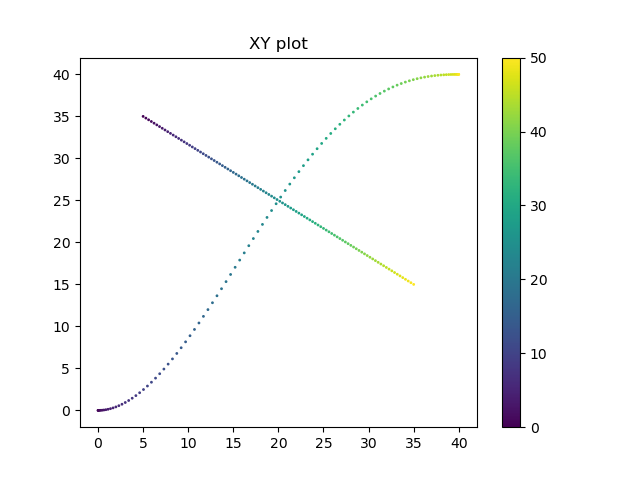
\includegraphics[width=\textwidth]{cc-cts-xy-plot.png}
        \caption{XY plots}
        \label{fig:sfig-cc-cts-e1-xy}
        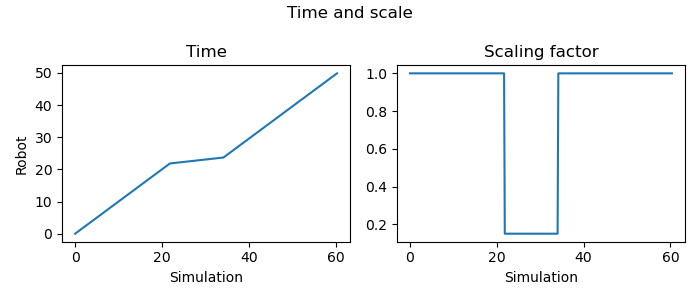
\includegraphics[width=\textwidth]{cc-cts-timescales.png}
        \caption{Time scaling}
        \label{fig:sfig-cc-cts-e1-ts}
    \end{subfigure}
    \begin{subfigure}[b]{0.49\textwidth}
        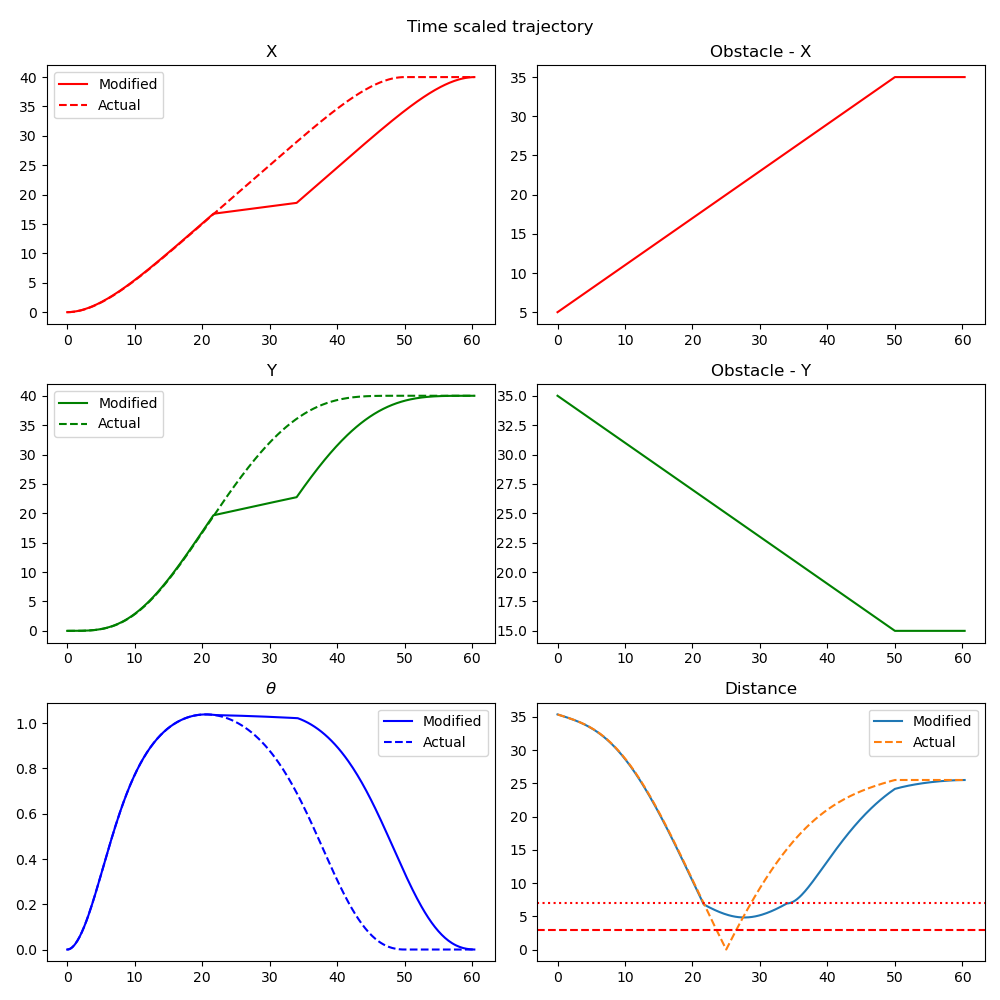
\includegraphics[width=\textwidth]{cc-cts-trajs.png}
        \caption{Time scaled results}
        \label{fig:sfig-cc-cts-e1-fgr}
    \end{subfigure}
    \caption{Collision cone based constant time scaling}
    \label{fig:cc-cts-exp1-graphs}
    \small
        The distance plot is shown in the bottom right of \ref{sub@fig:sfig-cc-cts-e1-fgr}. As seen, the time scaling gets activated at the thin red horizontal line (detection distance) and a collision is avoided (the distance plot does not cross the thick horizontal red line). See the slope and the scaling factor change in \ref{sub@fig:sfig-cc-cts-e1-ts}. The original (colliding) trajectories are shown in \ref{sub@fig:sfig-cc-cts-e1-xy}.
\end{figure}

\begin{figure}
    \centering
    \begin{subfigure}[b]{0.3\textwidth}
        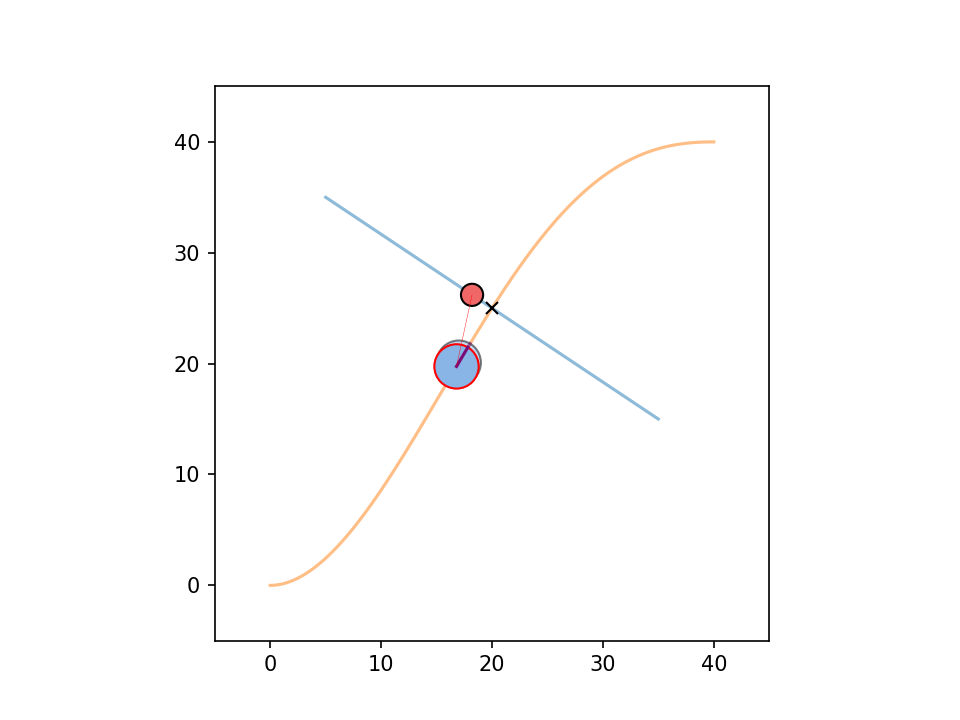
\includegraphics[width=\textwidth]{res2-ts-start.png}
        \caption{Start}
    \end{subfigure}
    \begin{subfigure}[b]{0.3\textwidth}
        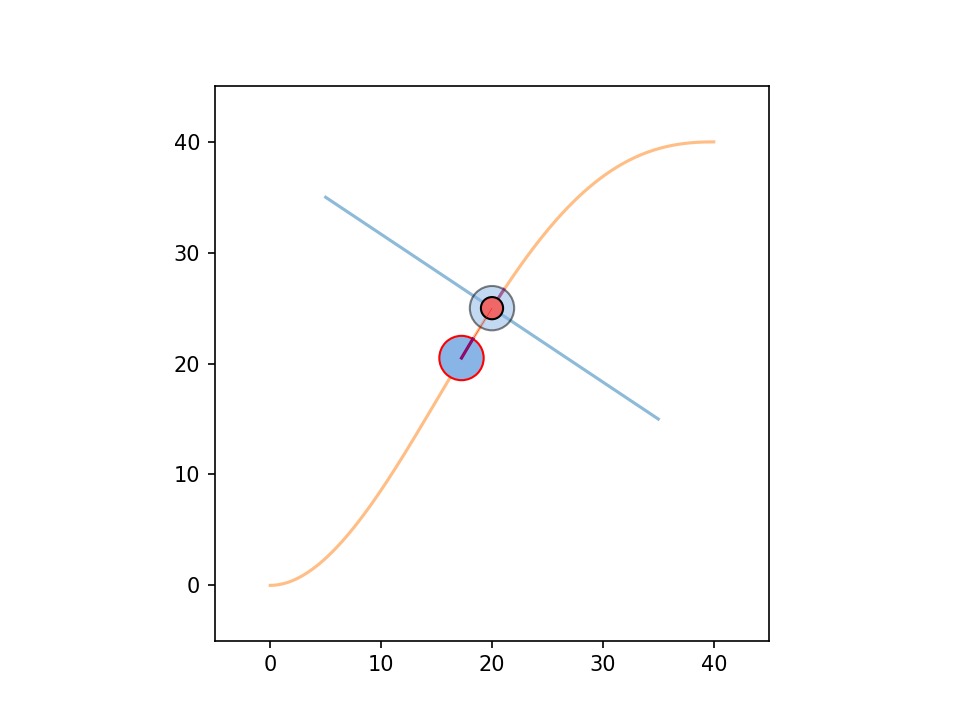
\includegraphics[width=\textwidth]{res2-ts-colav.png}
        \caption{Collision avoidance}
    \end{subfigure}
    \begin{subfigure}[b]{0.3\textwidth}
        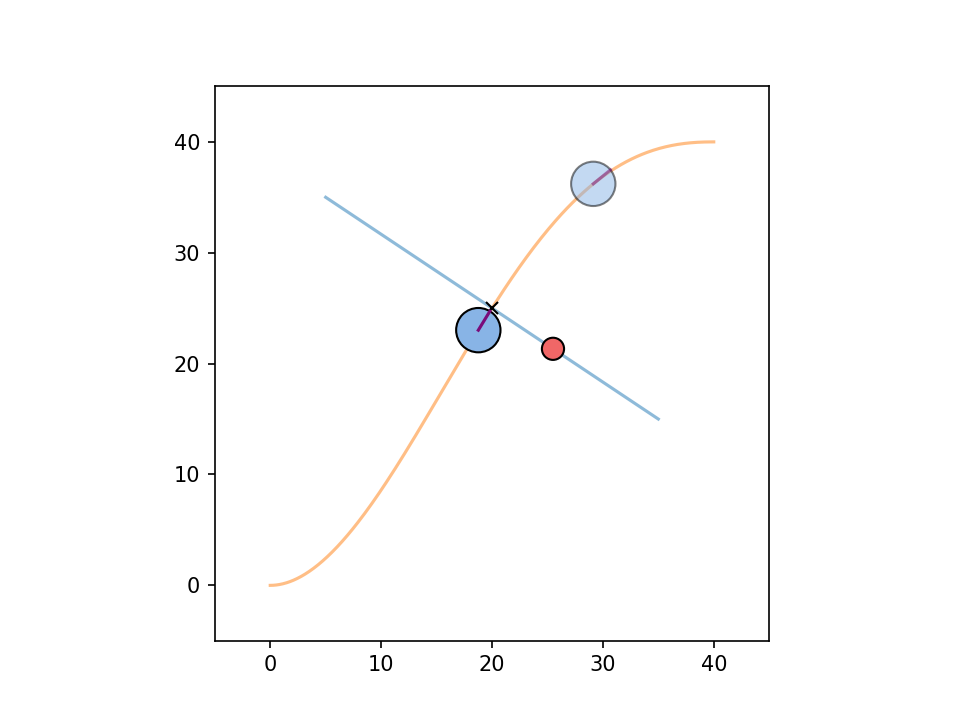
\includegraphics[width=\textwidth]{res2-ts-end.png}
        \caption{End}
    \end{subfigure}
    \caption{Collision cone - Constant time scaling - Video snaps}
    \label{fig:cc-cts-exp1}
\end{figure}

\subsubsection{Rule-based Linear time scaling}

We use the scaling factor as a function of the simulation time, given by $s(t) = a + bt$. The scaling is done as in constant time scaling case. The results are shown in figure \ref{fig:rb-lts-exp1-graphs}. The snippets from simulation are shown in figure \ref{fig:rb-lts-exp1}.

\begin{figure}
    \centering
    \begin{subfigure}[b]{0.49\textwidth}
        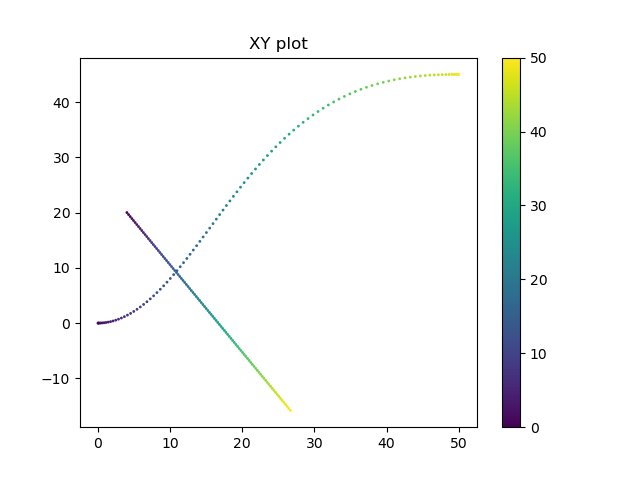
\includegraphics[width=\textwidth]{rb-lts-xy.png}
        \caption{XY plots}
        \label{fig:sfig-rb-lts-e1-xy}
        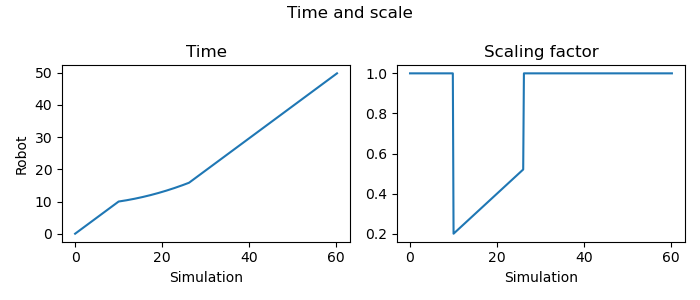
\includegraphics[width=\textwidth]{rb-lts-tscales.png}
        \caption{Time scaling}
        \label{fig:sfig-rb-lts-e1-ts}
    \end{subfigure}
    \begin{subfigure}[b]{0.49\textwidth}
        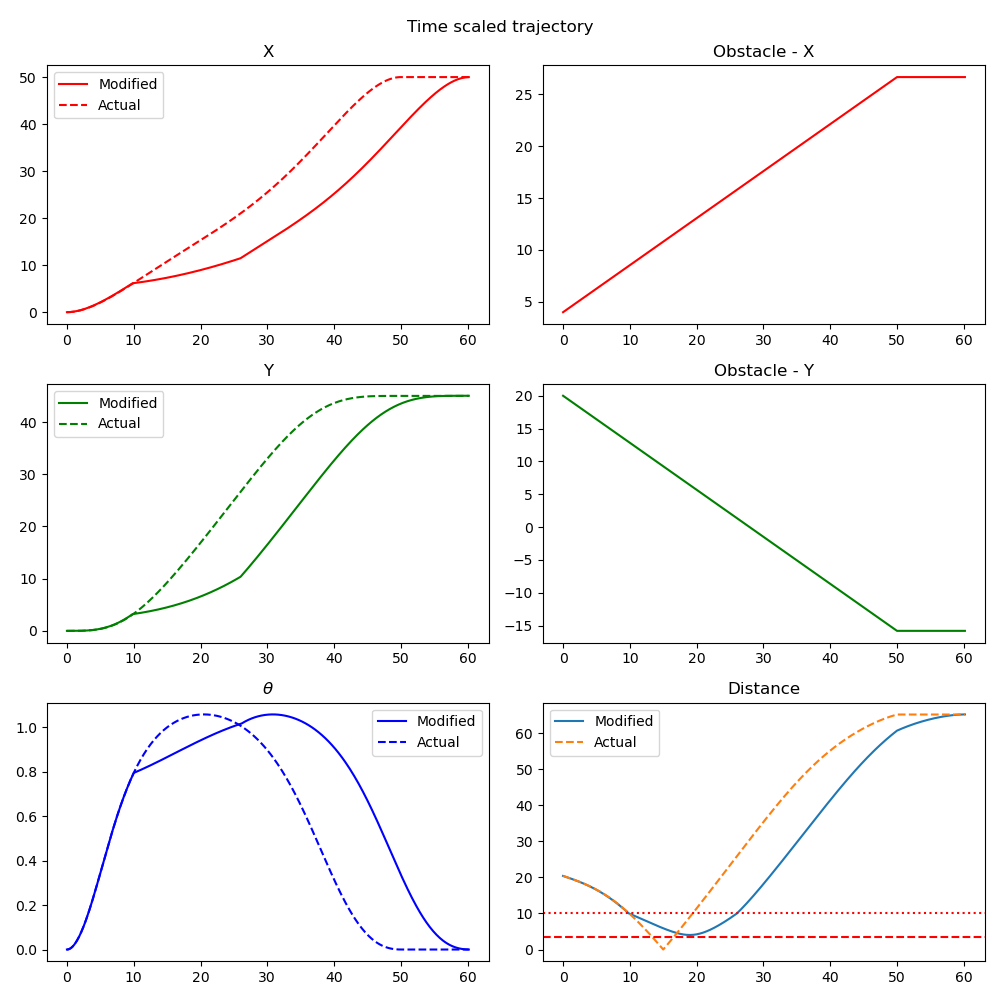
\includegraphics[width=\textwidth]{rb-lts-trajs.png}
        \caption{Time scaled results}
        \label{fig:sfig-rb-lts-e1-fgr}
    \end{subfigure}
    \caption{Rule-based Linear time scaling}
    \label{fig:rb-lts-exp1-graphs}
    \small
        The distance plot is shown in the bottom right of \ref{sub@fig:sfig-rb-lts-e1-fgr}. As seen, the time scaling gets activated at the thin red horizontal line (detection distance) and a collision is avoided (the distance plot does not cross the thick horizontal red line). See the slope and the scaling factor change in \ref{sub@fig:sfig-rb-lts-e1-ts} (notice the linear slope, with time as parabolic). The original (colliding) trajectories are shown in \ref{sub@fig:sfig-rb-lts-e1-xy}.
\end{figure}

\begin{figure}
    \centering
    \begin{subfigure}[b]{0.3\textwidth}
        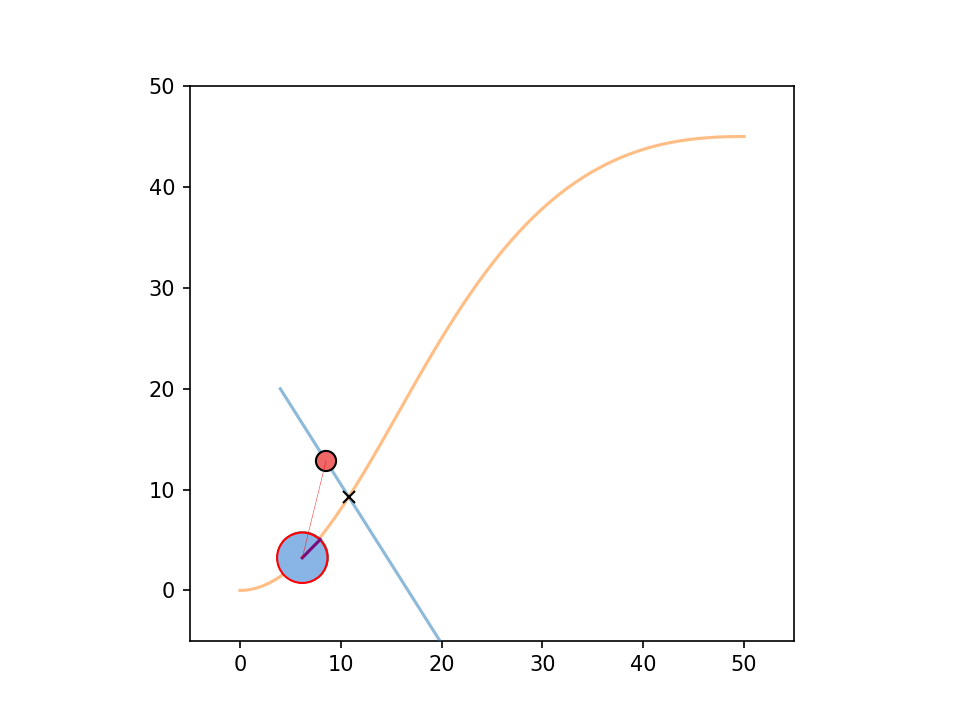
\includegraphics[width=\textwidth]{res3-ts-start.png}
        \caption{Start}
    \end{subfigure}
    \begin{subfigure}[b]{0.3\textwidth}
        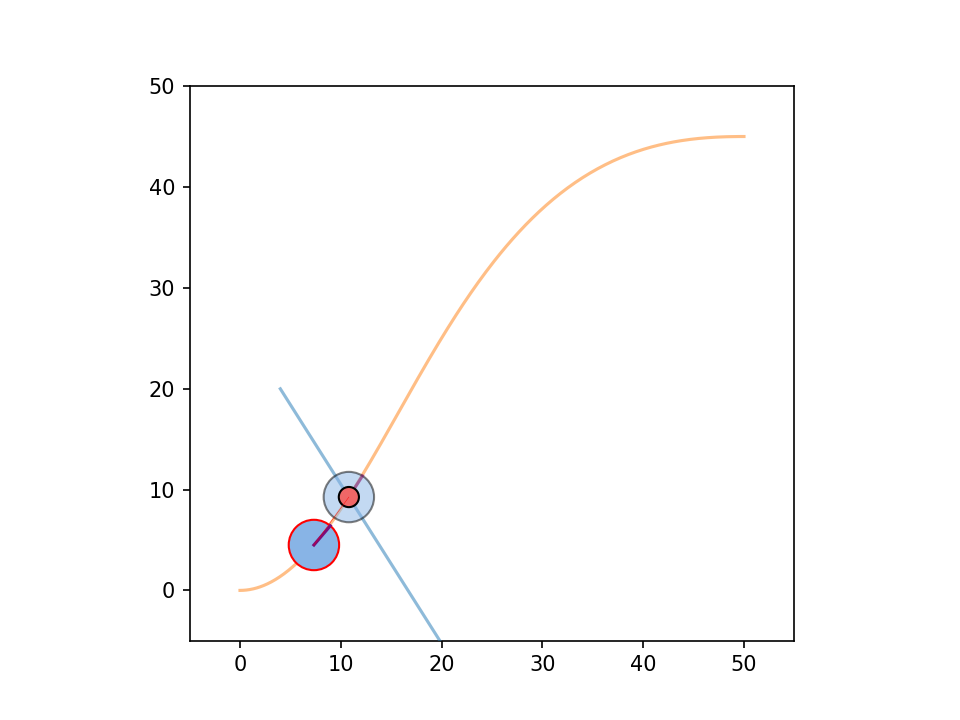
\includegraphics[width=\textwidth]{res3-ts-colav.png}
        \caption{Collision avoidance}
    \end{subfigure}
    \begin{subfigure}[b]{0.3\textwidth}
        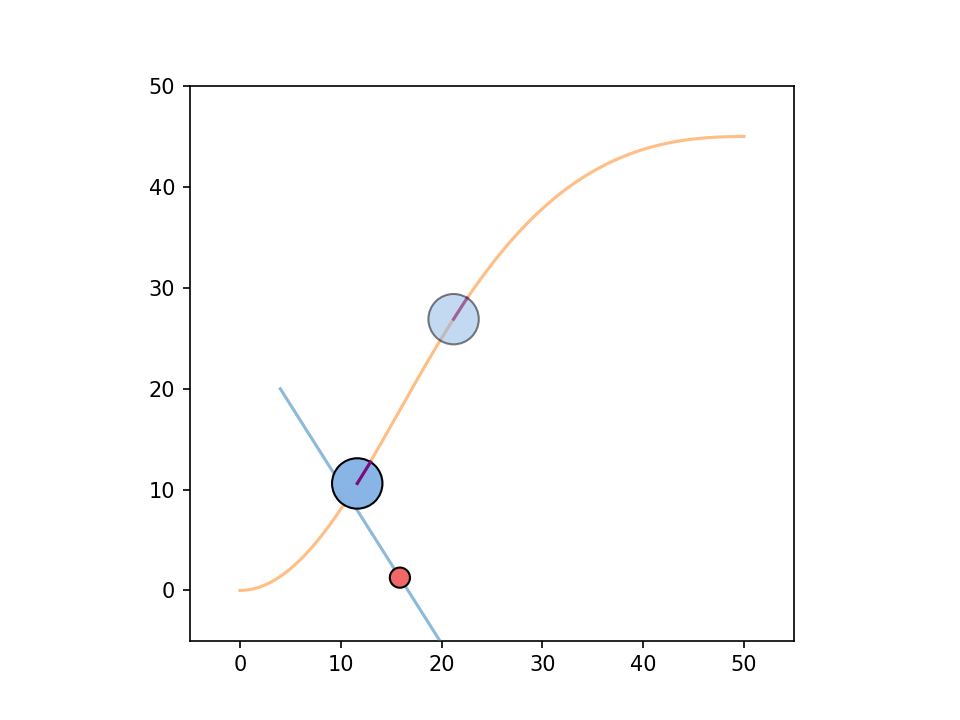
\includegraphics[width=\textwidth]{res3-ts-end.png}
        \caption{End}
    \end{subfigure}
    \caption{Rule-based - Linear time scaling - Video snaps}
    \label{fig:rb-lts-exp1}
    \small
        The simulation is available as \texttt{rb\_lts\_exp1.avi} in the \href{https://iiitaphyd-my.sharepoint.com/:f:/g/personal/avneesh_mishra_research_iiit_ac_in/Er_wRqK4hxVLjVdL56rfDxYBKr9PPed1laN48hLgLisf4w}{shared OneDrive folder}.
\end{figure}

\subsubsection{Smooth trajectory}

As we have seen, using iterative collision cone (in case of constant) and linear time scaling techniques did not completely fix the discontinuity problem. The following could be tried

\begin{itemize}
    \item Incorporate the acceleration and velocity constraints on the actuators. This way, even if the controller gives a time scaled velocity, the actuator will clip it towards the limits.
    
    However, this could be dangerous and could lead to collisions if the frequency of control loop isn't high enough or the constraints are too restrictive.
    
    \item Trajectories can be smoothened by incorporating information of higher derivatives in the time scaling problem.
    \item The entire problem could be converted into a constrained optimization problem, enforcing dynamic constraints.
    
    \item Some proposals include interleaving time-scaling with MPC \cite{tscc-mpc-2}, or using non-linear time scaling \cite{tscc-mpc-1} can also be used. 
\end{itemize}

\subsubsection{MPC Parallel}

Trajectories given by simple time-scaling (like what's implemented here) may not be very smooth, whereas trajectories from the MPC will be smooth (because it's from an optimizer using many more constraints on motion).

For the MPC to avoid collisions \emph{specifically} using time-scaling, you could add the time-scaling equations (like equation \ref{eq:cc-cts-rawineq}) as additional solver constraints and incorporate the scaling factor (or scaled velocities) in the system state (unknown variables). Otherwise, the MPC will deviate from the planned trajectory (to avoid the obstacle) whereas time-scaling will stay on the trajectory.

\subsubsection{Multi-robot}

Time scaling can be extended to multiple robots using an intersection space of multiple inequalities (as presented in \cite{rca-multirobot-rrc}). The solution space can be decomposed into multiple conditions (as done in \ref{eq:cc-cts-solspace-s}, but using different $a_i$ - one for each robot). 
Linear programming approaches can also solve such problems.

Using velocity obstacle \cite{fiorini98-vel-obs} is also a feasible solution (single robot and multiple obstacle case). The problem will more or less remain the same.

For any two robot case, the velocity vectors have to have sufficient deviation. If they're parallel or antiparallel, then time-scaling will not give a viable solution (it'll lead to collision or both remaining stationary). In such cases, path will have to be altered.
